\section{Analiza współczynników modyfikujących \newline średnią rozkładu}

Jako że współczynnik modyfikujący średnią rozkładu pozwolił na uzyskanie lepszych rezultatów niż do tej pory,
przeprowadzono badania dla różnych wartości parametru, wyniki są w plikach CSV na stronie \cite{research_results}.

Przeprowadzone zostały obliczenia dla następujących wartości modyfikatora: [0,1, 0,2, 0,5, 1, 2, 5, 10, 20, 50, 100, 200, 500, 1000],
oraz dla następujących wartości populacji: [20, 50, 100, 200, 500, 1000, 2000, 5000].

Niestety, niewiele z nich pozwoliło na uzyskanie więcej niż jednej grupy na wykresie. Wyniki przedstawiono na rysunkach
\ref{fig:watts_strogatz_10_20_8_student}, \ref{fig:barabasi_albert_2_20_2_student}, \ref{fig:barabasi_albert_2_50_2_student},
\ref{fig:erdos_renyi_10_50_8_student} i \ref{fig:watts_strogatz_10_20_7_student}.

\begin{figure}
    \centering
    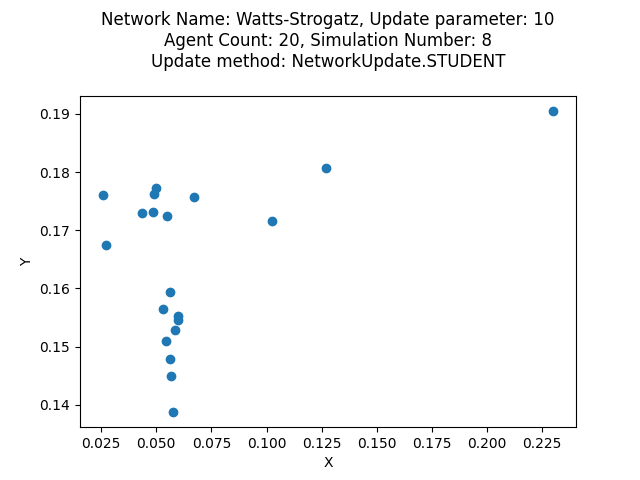
\includegraphics[width=0.5\textwidth]{img/watts_strogatz_10_20_8_student.png}
    \caption{Sieć Watts-Strogatz, parametr aktualizacji: 10, populacja: 20}
    \label{fig:watts_strogatz_10_20_8_student}
\end{figure}

\begin{figure}
    \centering
    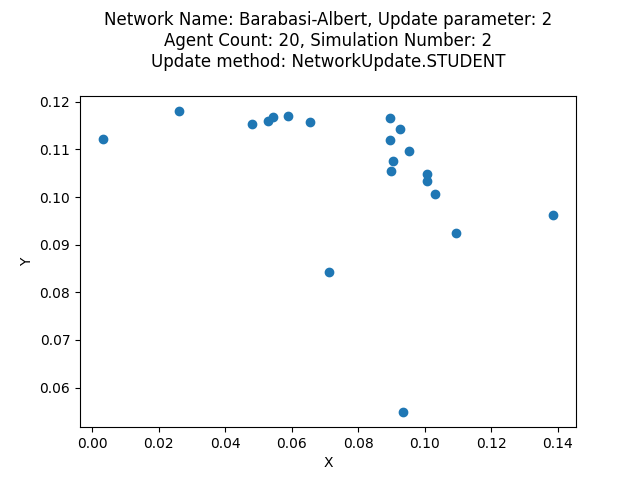
\includegraphics[width=0.5\textwidth]{img/barabasi_albert_2_20_2_student.png}
    \caption{Sieć Barabási-Albert, parametr aktualizacji: 2, populacja: 20}
    \label{fig:barabasi_albert_2_20_2_student}
\end{figure}

\begin{figure}
    \centering
    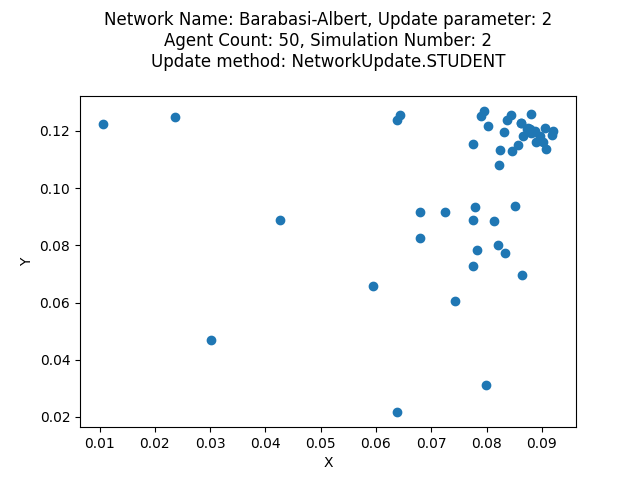
\includegraphics[width=0.5\textwidth]{img/barabasi_albert_2_50_2_student.png}
    \caption{Sieć Barabási-Albert, parametr aktualizacji: 2, populacja: 50}
    \label{fig:barabasi_albert_2_50_2_student}
\end{figure}

\begin{figure}
    \centering
    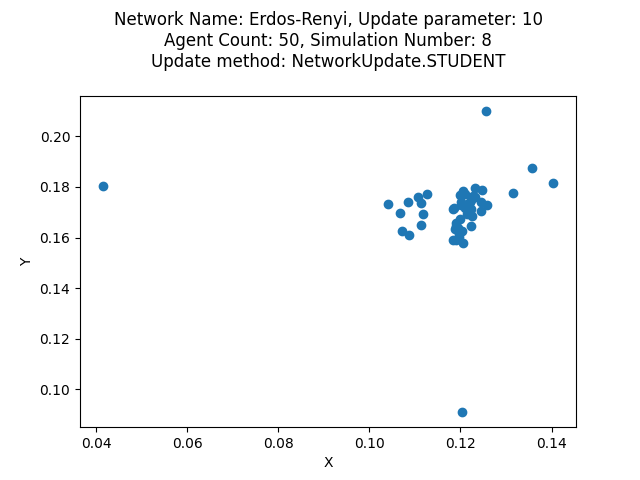
\includegraphics[width=0.5\textwidth]{img/erdos_renyi_10_50_8_student.png}
    \caption{Sieć Erdős-Rényi, parametr aktualizacji: 10, populacja: 50}
    \label{fig:erdos_renyi_10_50_8_student}
\end{figure}

\begin{figure}
    \centering
    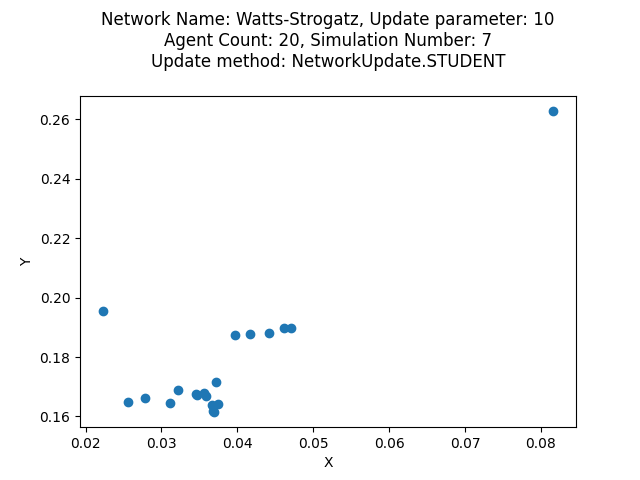
\includegraphics[width=0.5\textwidth]{img/watts_strogatz_10_20_7_student.png}
    \caption{Sieć Watts-Strogatz, parametr aktualizacji: 10, populacja: 20}
    \label{fig:watts_strogatz_10_20_7_student}
\end{figure}

